\documentclass[%
 aps,
 reprint,
 twocolumn,
%superscriptaddress,
%groupedaddress,
%unsortedaddress,
%runinaddress,
%frontmatterverbose, 
%preprint,
%preprintnumbers,
%nofootinbib,
%nobibnotes,
%bibnotes,
 amsmath,amssymb,
%  sor,
%  jor,
% pra,
% prb,
% rmp,
% prstab,
% prstper,
floatfix,
]{revtex4-2}

\usepackage{graphicx}% Include figure files
\usepackage{dcolumn}% Align table columns on decimal point
\usepackage{bm}% bold math
\usepackage[hidelinks]{hyperref}% add hypertext capabilities
\usepackage[mathlines]{lineno}% Enable numbering of text and display math
% \linenumbers\relax % Commence numbering lines
% \usepackage{unicode-math}

% \usepackage[showframe,%Uncomment any one of the following lines to test 
% %%scale=0.7, marginratio={1:1, 2:3}, ignoreall,% default settings
% %%text={7in,10in},centering,
% %%margin=1.5in,
% %%total={6.5in,8.75in}, top=1.2in, left=0.9in, includefoot,
% %%height=10in,a5paper,hmargin={3cm,0.8in},
% ]{geometry}
\usepackage[separate-uncertainty=true]{siunitx}
% \usepackage{caption}
% \usepackage{subcaption}
\usepackage{float}
\usepackage{enumitem}
\newcommand\tagthis{\addtocounter{equation}{1}\tag{\theequation}}
\newcommand{\Mod}{\ \mathrm{mod}\ }
\usepackage{physics}

\begin{document}

\preprint{APS/123-QED}

\title{Two-Ports Lossy Scattering in Quantum Optics}

\author{Randy Stefan Tanuwijaya}
\email{rstanuwijaya@connect.ust.hk}
\affiliation{
	Department of Physics \\
	The Hong Kong University of Science and Technology \\
	Clear Water Bay, Hong Kong
}

\date{\today}% It is always \today, today,
%  but any date may be explicitly specified

\begin{abstract}
	In this review we highlighted the difference between the classical and quantum probability for different input-output configurations in ideal and lossy scattering process for two-ports system. In the ideal scattering process, the classical probability significantly differs from the quantum probability due to the two-photons interference effect, where the probability of two photons outputs at different ports destructively interferes with each others. Whereas in the lossy scattering case, we derived an additional quantum correction term on top of the classical probability. Our investigation will be useful for the readers who are interested to understand how loss or absorption process may affect the probability on scattering process.
\end{abstract}
\maketitle

%\tableofcontents

\section{Introduction}
\label{sec:intro}
Quantum optics studies one of the most fundamental interactions in nature: light-matter interactions. The study of quantum optics has been a very active field of research for decades. It has led to many important discoveries, such as the demonstration of quantum entanglement through parametric down conversion \cite{perina_spontaneous_2014}, violation of Bell's inequality \cite{aspect_experimental_1982}, optical tweezers and laser cooling which led to the discovery of Bose-Einstein condensates \cite{wineland_radiation-pressure_1978, ashkin_acceleration_1970}. Quantum optics has also led to many critical applications, such as quantum communication, quantum computation, and quantum sensing \cite{lloyd_any_1992, ball_physicists_2020, yung_polarization_2022}.

Usually, when working with any quantum system, we simplify the case by assuming the system is ideal without any loss, which is not valid for real-world/experimental cases. This loss case has led to many interesting discussion around the Parity-Time symmetry \cite{minganti_quantum_2019,arkhipov_liouvillian_2020}. Recent discussions in lossy/non-Hermitian quantum systems address this issue, which develops a framework that includes the loss and gain in a given quantum system \cite{leonhardt_quantum_2003, wong_quantum_2022}. In particular, for a quantum optical system, we define the loss and gain of our system as separate modes in the ancilla mode.

In this review, we derive and highlight the important parameters to characterize two-ports lossy scattering, such as the quantum probability for each input-output configuration, and compare it with the classical probability. To do so, we will first introduce the concept of Fock space and scattering operator to define our system's quantum state and transformation. Then, we will discuss the ideal case without photon loss. In this case, the quantum probability will significantly differ from the classical one due to the two-photon interference effect \cite{hong_measurement_1987}. Finally, we will discuss the probability of photon absorption and derive a correction term for quantum probability.

\begin{section}{Results}
\label{sec:methodology}

\subsection{Fock Space}
To describe the quantum optical system, we use the Fock space representation. The Fock space representation is a convenient representation for the Hilbert space of the quantum optical system. Instead of using quantized energy levels, the Fock space representation uses the number of photons in the system. Similar to the ladder methods, we can define the creation and annihilation operators for the Fock space representation. The creation operator $\hat{a}_i^\dagger$ and annihilation operator $\hat{a}_i$ are defined as:

\begin{subequations}
	\begin{eqnarray}
		\hat{a}_i^\dagger\ket{n_i}     & = \sqrt{n_i+1}\ket{n_i+1}
		\\
		\hat{a}_i\ket{n_i} & = \sqrt{n_i}\ket{n_i-1}
		\\
		\left[ \hat{a}_i \hat{a}_j^\dagger \right]   & = \delta_{ij}
	\end{eqnarray}
\end{subequations}
where $n_i$ is the number of photons in the $i$-th mode.

Usually, the system have many different modes, i.e. forward $n_f$ and backward $n_b$ propagation mode, polarizations mode ($n_x$ and $n_y$), and ancilla mode ($n'_i$, $n'_j$, ...). Using this definition, we can define the two different modes in our system, such as:
\begin{enumerate}
	\item {\bf radiation mode}, which is the mode that the radiation propagates in, and the state in this mode is independently measurable. For example, we can measure the polarization and the propagation mode independently.
	\item {\bf ancilla mode}, which is defined as the modes that are not used to propagate the light, such as photon absorption or emission within the system. Thus, we cannot measure the state of the ancilla mode directly.
\end{enumerate}
Finally, we can define the fock space for each mode to be the basis for the system fock space, such as:
\begin{align*}
	\ket{\psi} = \ket{n_{fx}, n_{fy}, n_{bx}, n_{by}, \dots, n'_{i}, n'_{j}, \dots}
\end{align*}

One important properties of this fock space representation is that we can express any state by applying the creation operator many times to the vacuum state. For example, the state $\ket{n}$ can be expressed as:
\begin{align*}
	\ket{n} = \frac{1}{\sqrt{n!}} (\hat{a}^\dagger)^n \ket{0}
\end{align*}

\subsection{Scattering Matrix}
In the ideal case, optical components which affect the propagation of the light can be described using the unitary scattering matrix $\hat{U} \equiv \hat{S}_{all}$ which include both radiation mode and ancilla mode. Moreover, is often convenient to describe the system in the Heisenberg picture, in which the operator will undergo a unitary transformation under $\hat{U}$ after the light has passed through the scattering material. For example, consider the following scattering process, where the creation operator changes from $\hat{a}_{i, in}$ to $\hat{a}_{i, out}$:
\begin{align*}
	\hat{a}_{i, out} & = \hat{U} \hat{a}_{i, in} \hat{U}^\dagger = \sum_{j} U_{ij} \hat{a}_j \tagthis \label{eq:heisenberg} \\
	                 & = \sum_{j \in rad} U_{ij} \hat{a}_j  + \sum_{j' \in anc} U_{ij'} \hat{a}_{j'}
\end{align*}
where the first term $j$ sums over the radiation mode and the second term $j'$ sums over the ancilla modes.

However, in the real-world scenario, the scattering matrix is generally not unitary. In this case, we can define the scattering matrix which only include the radiation mode as:
\begin{align}
	\hat{S} \equiv \bra{0_{anc}} \hat{U} \ket{0_{anc}}
\end{align}
where $\ket{0_{anc}}$ denote 0 photon input in ancilla mode and $\bra{0_{anc}}$ denotes 0 photon output in ancilla mode. Essentially, this is the subspace of the unitary scattering matrix where the ancilla mode is not used in by the scattering process.

It is often useful to define the commutation relation between the scattering matrix and the creation and annihilation operators. We can start by considering Eq. \ref{eq:heisenberg} \cite{leonhardt_quantum_2003}:
\begin{align*}
	\hat{U} \hat{a}_i^\dagger \hat{U}^\dagger & = \sum_{j} U_{ij} \hat{a}_j^\dagger         \\
	\hat{U} \hat{a}_i^\dagger           & = \sum_{j} U_{ij} \hat{a}_j^\dagger \hat{U}
\end{align*}

Similarly, for radiation mode scattering matrix, we can also define the following relation between the scattering matrix and the creation and annihilation operators, in which case we make use of the Lindblad master equation, which is a time-differential equation on the density matrix of the interested subspace \cite{minganti_quantum_2019,arkhipov_liouvillian_2020}:
\begin{align*}
	\text{propagation} &  & \hat{S}\hat{a_k}^\dagger & = \sum_i \hat{a_i}^\dagger S_{ik} \hat{S} \tagthis \label{eq:propagation} \\
	\text{measurement} &  & \hat{a_k}\hat{S}   & = \sum_i \hat{a_i} S_{ki} \hat{S}^\dagger \tagthis \label{eq:measurement}
\end{align*}
In particular, the above relation is useful to describe the propagation and measurement process in the system.

\subsection{Ideal Two-Ports System}
One particular system that we will be studying is the two ports system. The two ports system is a system that has two input ports and two output ports. Such system can be described using the $2 × 2$ scattering-matrix. First, we can make use of these useful relations by using Eq. \ref{eq:propagation} and Eq. \ref{eq:measurement}:
\begin{align*}
	\bra{0}\hat{a}_{i}\hat{S}\hat{a}_{i'}^\dagger\ket{0}                                & = S_{ii'}                         \\
	\bra{0}\hat{a}_{i}\hat{a}_{j}\hat{S}\hat{a}_{i'}^\dagger\hat{a}_{j'}^\dagger\ket{0} & = S_{ii'}S_{jj'} + S_{ij'}S_{ji'}
\end{align*}

For example, we use the above relation to calculate the probablility amplitude of the following input-output configurations:
\begin{align*}
	\bra{1_i} \hat{S} \ket{1_k}         & = \bra{0} \hat{a}_i \hat{S} \hat{a}_k^\dagger \ket{0}                                                \\
	                                    & = S_ik                                                                                               \\
	\bra{1_1 1_2} \hat{S} \ket{1_1 1_2} & = \bra{0} \hat{a}_1 \hat{a}_2 \hat{S} \hat{a}_1^\dagger \hat{a}_2^\dagger \ket{0}                    \\
	                                    & = S_{11}S_{22} + S_{12}S_{21}                                                                        \\
	\bra{2_1 0_2} \hat{S} \ket{1_1 1_2} & = \frac{1}{\sqrt{2}} \bra{0} \hat{a}_1 \hat{a}_1 \hat{S} \hat{a}_1^\dagger \hat{a}_2^\dagger \ket{0} \\
	                                    & = \frac{1}{\sqrt{2}} (S_{11} S_{12} + S_{11} S_{12})                                                 \\
	                                    & = \sqrt{2} (S_{11} S_{12})                                                                           \\
	\bra{0_1 2_2} \hat{S} \ket{1_1 1_2} & = \sqrt{2} (S_{21} S_{22})
\end{align*}

Some example of two ports system includes: (unpolarized) beam splitter, linear polarizer, quarter wave plates, and half wave plate. For example, the scattering matrix of an {\bf ideal beam splitter} is given by:
\begin{align*}
	\hat{S} = \hat{U} = \frac{1}{\sqrt{2}} \begin{pmatrix}
		                                       1 & i \\
		                                       i & 1
	                                       \end{pmatrix}
\end{align*}
For one photon comming in to each port, it gives us the following probablility:
\begin{align*}
	P(1_1 1_2 | 1_1 1_2) = \left| \bra{1_1 1_2} \hat{S} \ket{1_1 1_2} \right|^2 & = 0   \\
	P(2_1 0_2 | 1_1 1_2) = \left| \bra{2_1 0_2} \hat{S} \ket{1_1 1_2} \right|^2 & = 1/2 \\
	P(0_1 2_2 | 1_1 1_2) = \left| \bra{0_1 2_2} \hat{S} \ket{1_1 1_2} \right|^2 & = 1/2
\end{align*}
These results significantly differ from the classical case, in which the probabilities are given by: $P_c(1_1 1_2 | 1_1 1_2) = 1/2$ and $P_c(2_1 0_2 | 1_1 1_2) = P_c(0_1 2_2 | 1_1 1_2) = 1/4$.

Given that the two photons are indistinguishable and arrives at the beam splitter at the same time, the probability of the input-output configuration $(1_1 1_2| 1_1 1_2)$ is 0, i.e. the photons will be bunched together to the same output. This is known as the famous two-photon intererence effect or the {\bf Hong-Ou-Mandel (HOM)} effect \cite{hong_measurement_1987}, which is a very important effect in quantum optics and quantum information. The experimental verification of the HOM effect is shown in Fig. The HOM effect enables quantum information processing for linear optical quantum computing system (LOQC).

\begin{figure}
	\centering
	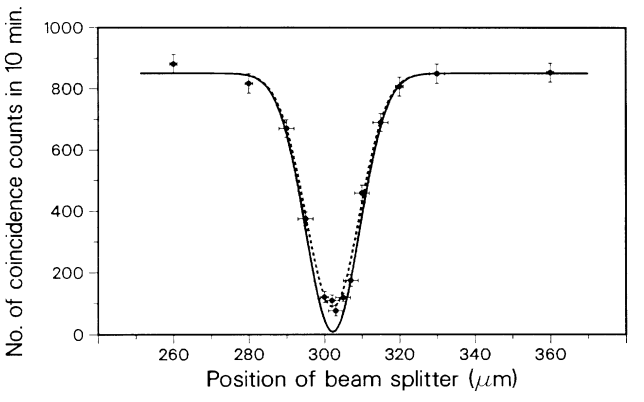
\includegraphics[width=\linewidth]{figures/hom.png}
	\caption{Experimental verification of the HOM effect \cite{hong_measurement_1987}. The x-axis is the delay distance between the two input ports, and the y-axis is the number of coincident photon, i.e. detection of photons coming out from both ports at the same time. The number coincidence drops to zero when the optical path of the two ports are exactly the same, corresponding to the $P(1_1 1_2 | 1_1 1_2) = 0$.}
	\label{fig:hom}
\end{figure}

\subsection{Lossy/Non-Hermitian Two-Ports System}
For a lossy system, we must take account of the ancilla mode of the system. Thus, the system is no longer only described by two-modes, but 2-radiation modes and infinitely many ancilla mode (loss channel and 0 gain channel).

First, we can define the absorption efficiency (probability of absorption) of each input port $j$ in our system as $A_j$ as:
\begin{align}
	A_j = 1 - \sum_{i} |S_{ij}|^2 \tagthis \label{eq:absorption}
\end{align}

For example, the simple case of 1 photon in input port $j$ gives the following scattering probability:
\begin{align}
	P(1_i | 1_j) & = \left| \bra{0} \hat{a}_i \hat{S} \hat{a}_j^\dagger \ket{0} \right|^2 = \left| S_{ij} \right|^2 \\
	P(0 | 1_j)   & = \sum_{i} |R_{ij}|^2  = 1 - \sum_{i} |S_{ij}|^2 = A_j
\end{align}
where $\hat{R}$ is the subspace of unitary scattering matrix $U$ that corresponds to the loss channel, i.e. $\hat{R} = \bra{0_{rad}} \hat{U} \ket{0_{anc}}$.

For two photons input, we can still make use of our previous result. For example, consider the case where the input-output configurations are $(1_1 | 1_1 1_2)$ and $(0 | 1_1 1_2)$, i.e. one or two photon(s) got absorbed.
\begin{align*}
	P(1_1 &| 1_1 1_2)  = \sum_i \left| S_{11} R_{i2} + R_{i1} S_{12} \right|^2 \\
	                  &= |S_{11}|^2 A_2 + |S_{12}|^2 A_1 - 2 \Re\left( S_{11}^* S_{12} \sum_i  S_{i2}^* S_{i1} \right)                               
\end{align*}
\begin{align*}
	P(0 | 1_1 1_2) & = \frac{1}{2} \sum_i \sum_j \left| R_{i1} R_{j2} + R_{j1} R_{i2} \right|^2  \\
	               & = A_1A_2 + \Re\left( \sum_i S_{i1}^* S_{i2} \sum_j S_{j2}^* S_{j1}  \right)
\end{align*}
We can see the additional terms is due to the quantum interference effect. In particular, the classical probabilities are: $P_c(1_1 | 1_1 1_2) = |S_{11}|^2 A_2 + |S_{12}|^2 A_1$ and $P_c(0 | 1_1 1_2) = A_1A_2$. 
\end{section}

\bigskip
\section{Conclusion}
This article highlights the key difference between the classical and quantum probability for the ideal and lossy scattering two-ports system. First, model the scattering process as a unitary transformation in the Heisenberg system. Furthermore, we have derived the two-photon/HOM interference effect for the beam splitter and the quantum correction terms for the photon absorption in the lossy two-ports system. Moreover, the mathematical framework we are working in this article can be extended to any arbitrary number of ports in the systems, not only limited for two-ports system. We believe this article will be helpful for readers who are interested to learn more about the lossy scattering process in quantum optical systems.

\bibliography{bibliography}
\begin{widetext}
	\section*{Appendix}
	\subsection{Lossy Two-Ports System}
	\begin{align*}
		P(1_1 | 1_1 1_2) & = \sum_i \left| S_{11} R_{i2} + R_{i1} S_{12} \right|^2                                                                       \\
		                 & = |S_{11}|^2 \sum_i |R_{i2}|^2 + |S_{12}|^2  \sum_{i} |R_{i1}|^2 + 2 \Re\left( \sum_i S_{11}^* S_{i2}^* S_{i1} S_{12} \right) \\
		                 & = |S_{11}|^2 A_2 + |S_{12}|^2 A_1 + 2 \Re\left( S_{11}^* S_{12} \sum_i  R_{i2}^* R_{i1} \right)                               \\
		                 & = |S_{11}|^2 A_2 + |S_{12}|^2 A_1 - 2 \Re\left( S_{11}^* S_{12} \sum_i  S_{i2}^* S_{i1} \right)                               \\
		                 & = |S_{11}|^2 A_2 + |S_{12}|^2 A_1 - 2 \Re\left( S_{11}^* S_{12} (S_{12}^* S_{11} + S_{22}^* S_{21}) \right)                   \\
						 \\
	% \end{align*}
	% \begin{align*}
		P(0 | 1_1 1_2) & = \sum_i \sum_{j > i} \left| R_{i1} R_{j2} + R_{j1} R_{i2} \right|^2 = \frac{1}{2} \sum_i \sum_j \left| R_{i1} R_{j2} + R_{j1} R_{i2} \right|^2 \\
		               & = \frac{1}{2} \sum_i \sum_j |R_{i1}|^2 |R_{j2}|^2 + |R_{j1}|^2 |R_{i2}|^2 + 2 \Re\left( R_{i1}^* R_{j2}^* R_{j1} R_{i2} \right)                 \\
		               & = A_1A_2 + \Re\left( \sum_i R_{i1}^* R_{i2} \sum_j R_{j2}^* R_{j1}  \right)                                                                     \\
		               & = A_1A_2 + \Re\left( \sum_i R_{i1}^* R_{i2} \sum_j R_{j2}^* R_{j1}  \right)                                                                     \\
		               & = A_1A_2 + \Re\left( \sum_i S_{i1}^* S_{i2} \sum_j S_{j2}^* S_{j1}  \right)                                                                     \\
		               & = A_1A_2 + \Re\left( (S_{11}^* S_{12} + S_{21}^* S_{22}) (S_{12}^* S_{11} + S_{22}^* S_{21})  \right)                                           \\
	\end{align*}
\end{widetext}

\end{document}
%
% ****** End of file apssamp.tex ******
